%% BioMed_Central_Tex_Template_v1.06
%%                                      %
%  bmc_article.tex            ver: 1.06 %
%                                       %

%%IMPORTANT: do not delete the first line of this template
%%It must be present to enable the BMC Submission system to
%%recognise this template!!

%%%%%%%%%%%%%%%%%%%%%%%%%%%%%%%%%%%%%%%%%
%%                                     %%
%%  LaTeX template for BioMed Central  %%
%%     journal article submissions     %%
%%                                     %%
%%          <8 June 2012>              %%
%%                                     %%
%%                                     %%
%%%%%%%%%%%%%%%%%%%%%%%%%%%%%%%%%%%%%%%%%

%%%%%%%%%%%%%%%%%%%%%%%%%%%%%%%%%%%%%%%%%%%%%%%%%%%%%%%%%%%%%%%%%%%%%
%%                                                                 %%
%% For instructions on how to fill out this Tex template           %%
%% document please refer to Readme.html and the instructions for   %%
%% authors page on the biomed central website                      %%
%% https://www.biomedcentral.com/getpublished                      %%
%%                                                                 %%
%% Please do not use \input{...} to include other tex files.       %%
%% Submit your LaTeX manuscript as one .tex document.              %%
%%                                                                 %%
%% All additional figures and files should be attached             %%
%% separately and not embedded in the \TeX\ document itself.       %%
%%                                                                 %%
%% BioMed Central currently use the MikTex distribution of         %%
%% TeX for Windows) of TeX and LaTeX.  This is available from      %%
%% https://miktex.org/                                             %%
%%                                                                 %%
%%%%%%%%%%%%%%%%%%%%%%%%%%%%%%%%%%%%%%%%%%%%%%%%%%%%%%%%%%%%%%%%%%%%%

%%% additional documentclass options:
%  [doublespacing]
%  [linenumbers]   - put the line numbers on margins

%%% loading packages, author definitions

%\documentclass[twocolumn]{bmcart}% uncomment this for twocolumn layout and comment line below
\documentclass{bmcart}

%%% Load packages
\usepackage{array}
\usepackage{amsthm,amsmath}
%\RequirePackage[numbers]{natbib}
%\RequirePackage[authoryear]{natbib}% uncomment this for author-year bibliography
%\RequirePackage{hyperref}
\usepackage[utf8]{inputenc} %unicode support
%\usepackage[applemac]{inputenc} %applemac support if unicode package fails
%\usepackage[latin1]{inputenc} %UNIX support if unicode package fails
\usepackage{graphicx}
%%%%%%%%%%%%%%%%%%%%%%%%%%%%%%%%%%%%%%%%%%%%%%%%%
%%                                             %%
%%  If you wish to display your graphics for   %%
%%  your own use using includegraphic or       %%
%%  includegraphics, then comment out the      %%
%%  following two lines of code.               %%
%%  NB: These line *must* be included when     %%
%%  submitting to BMC.                         %%
%%  All figure files must be submitted as      %%
%%  separate graphics through the BMC          %%
%%  submission process, not included in the    %%
%%  submitted article.                         %%
%%                                             %%
%%%%%%%%%%%%%%%%%%%%%%%%%%%%%%%%%%%%%%%%%%%%%%%%%

%%%%% UN COMMENT BEFORE SUBMISSION
%\def\includegraphic{}
%\def\includegraphics{}

%%% Put your definitions there:
\startlocaldefs
\endlocaldefs

%%% Begin ...
\begin{document}

%%% Start of article front matter
\begin{frontmatter}

\begin{fmbox}
\dochead{Research}

%%%%%%%%%%%%%%%%%%%%%%%%%%%%%%%%%%%%%%%%%%%%%%
%%                                          %%
%% Enter the title of your article here     %%
%%                                          %%
%%%%%%%%%%%%%%%%%%%%%%%%%%%%%%%%%%%%%%%%%%%%%%

\title{Evaluating trait-based sets for taxonomic enrichment analysis applied to human microbiome data sets}

%%%%%%%%%%%%%%%%%%%%%%%%%%%%%%%%%%%%%%%%%%%%%%
%%                                          %%
%% Enter the authors here                   %%
%%                                          %%
%% Specify information, if available,       %%
%% in the form:                             %%
%%   <key>={<id1>,<id2>}                    %%
%%   <key>=                                 %%
%% Comment or delete the keys which are     %%
%% not used. Repeat \author command as much %%
%% as required.                             %%
%%                                          %%
%%%%%%%%%%%%%%%%%%%%%%%%%%%%%%%%%%%%%%%%%%%%%%

\author[
  addressref={aff1,aff2},                   
  email={quang.p.nguyen.gr@dartmouth.edu}   % email address
]{\inits{Q.P.N.}\fnm{Quang P.} \snm{Nguyen}}
\author[
  addressref={aff1,aff2},
  email={anne.g.hoen@dartmouth.edu}
]{\inits{A.G.H.}\fnm{Anne G.} \snm{Hoen}}
\author[
  addressref={aff1},
  corref={aff1},
  email={hildreth.r.frost@dartmouth.edu}
]{\inits{H.R.F.}\fnm{H. Robert} \snm{Frost}}

%%%%%%%%%%%%%%%%%%%%%%%%%%%%%%%%%%%%%%%%%%%%%%
%%                                          %%
%% Enter the authors' addresses here        %%
%%                                          %%
%% Repeat \address commands as much as      %%
%% required.                                %%
%%                                          %%
%%%%%%%%%%%%%%%%%%%%%%%%%%%%%%%%%%%%%%%%%%%%%%

\address[id=aff1]{%                           % unique id
  \orgdiv{Department of Biomedical Data Science},             % department, if any
  \orgname{Dartmouth College},          % university, etc
  \city{Hanover},                              % city
  \cny{NH, USA}                                    % country
}
\address[id=aff2]{%
  \orgdiv{Department of Epidemiology},
  \orgname{Dartmouth College},
  %\street{},
  %\postcode{}
  \city{Hanover},
  \cny{NH, USA}
}

%%%%%%%%%%%%%%%%%%%%%%%%%%%%%%%%%%%%%%%%%%%%%%
%%                                          %%
%% Enter short notes here                   %%
%%                                          %%
%% Short notes will be after addresses      %%
%% on first page.                           %%
%%                                          %%
%%%%%%%%%%%%%%%%%%%%%%%%%%%%%%%%%%%%%%%%%%%%%%

%\begin{artnotes}
%%\note{Sample of title note}     % note to the article
%\note[id=n1]{Equal contributor} % note, connected to author
%\end{artnotes}

\end{fmbox}% comment this for two column layout

%%%%%%%%%%%%%%%%%%%%%%%%%%%%%%%%%%%%%%%%%%%%%%%
%%                                           %%
%% The Abstract begins here                  %%
%%                                           %%
%% Please refer to the Instructions for      %%
%% authors on https://www.biomedcentral.com/ %%
%% and include the section headings          %%
%% accordingly for your article type.        %%
%%                                           %%
%%%%%%%%%%%%%%%%%%%%%%%%%%%%%%%%%%%%%%%%%%%%%%%

\begin{abstractbox}

\begin{abstract} % abstract
\parttitle{Background} Set-based pathway analysis is a powerful tool that allows researchers to summarize complex genomic variables in the form of biologically interpretable sets. Since the microbiome is characterized by a high degree of inter-individual variability in taxonomic compositions, applying enrichment methods using on functionally driven taxon sets can increase both the reproducibility and interpretability of microbiome association studies. However, there is still an open question of which knowledge base to utilize for set construction. Here, we evaluate microbial trait databases, which aggregates experimentally determined microbial phenotypes, as a potential avenue for meaningful construction of taxon sets.  

\parttitle{Methods} Using publicly available microbiome sequencing data sets (both 16S rRNA gene metabarcoding and whole-genome metagenomics), we assessed these trait-based sets on three aspects: first, do they cover the diversity of microbes obtained from a typical data set, and second, do they confer additional predictive power on disease prediction tasks when assessed against measured pathway abundances and PICRUSt2 prediction.   
%third, for sets that are found to be enriched, are pathways corresponding to the trait also have increased abundances.     

\parttitle{Results} 
\parttitle{Conclusions}

\end{abstract}

%%%%%%%%%%%%%%%%%%%%%%%%%%%%%%%%%%%%%%%%%%%%%%
%%                                          %%
%% The keywords begin here                  %%
%%                                          %%
%% Put each keyword in separate \kwd{}.     %%
%%                                          %%
%%%%%%%%%%%%%%%%%%%%%%%%%%%%%%%%%%%%%%%%%%%%%%

\begin{keyword}
\kwd{microbiome}
\kwd{enrichment analysis}
\kwd{trait-based analysis}
\end{keyword}

% MSC classifications codes, if any
%\begin{keyword}[class=AMS]
%\kwd[Primary ]{}
%\kwd{}
%\kwd[; secondary ]{}
%\end{keyword}

\end{abstractbox}
%
%\end{fmbox}% uncomment this for two column layout

\end{frontmatter}

%%%%%%%%%%%%%%%%%%%%%%%%%%%%%%%%%%%%%%%%%%%%%%%%
%%                                            %%
%% The Main Body begins here                  %%
%%                                            %%
%% Please refer to the instructions for       %%
%% authors on:                                %%
%% https://www.biomedcentral.com/getpublished %%
%% and include the section headings           %%
%% accordingly for your article type.         %%
%%                                            %%
%% See the Results and Discussion section     %%
%% for details on how to create sub-sections  %%
%%                                            %%
%% use \cite{...} to cite references          %%
%%  \cite{koon} and                           %%
%%  \cite{oreg,khar,zvai,xjon,schn,pond}      %%
%%                                            %%
%%%%%%%%%%%%%%%%%%%%%%%%%%%%%%%%%%%%%%%%%%%%%%%%

%%%%%%%%%%%%%%%%%%%%%%%%% start of article main body
% <put your article body there>

%%%%%%%%%%%%%%%%
%% Background %%
%%
\section*{Introduction}

Advancements in high-throughout sequencing technologies have allowed researchers to characterize the identity and functional potential of a large proportion of microorganisms in human-associated microbiomes. This has enabled efficient study of the link between health outcomes and the microbiota without reliance on currently limited culture-based approaches \cite{lagier2016culture}. As such, there has been an increase in microbiome profiling studies, primarily aiming towards identifying specific microbes that are differentially abundant across healthy controls and diseased individuals \cite{zhang2019advancing}. However, such analyses face unique computational and statistical challenges \cite{li2019statistical}, which includes addressing the burden of multiple testing and providing meaningful biological interpretations.  

\noindent This issue of understanding obtained results in the broader context of biological processes mirrors that of other high-throughput data sets. One approach that has proven to be fruitful in human genomic studies is gene set testing (or pathway analysis) which focuses on analyzing the coordinated expression of groups of genes (termed gene sets) \cite{maleki2020gene}. Since these gene sets are usually defined in terms of biological annotations \cite{liberzon2015molecular}, results are often more interpretable and more powered compared to a gene-centric approach \cite{goeman2007analzying}.   



\section*{Material and methods}

All analyses were performed in the R programming language (version 4.1.2) \cite{rcoreteam2021language} and the Python programming language (version 3.10.4). All graphics were generated using \texttt{ggplot2}, \texttt{ggsci}, \texttt{patchwork}. Tabular data manipulation was performed using \texttt{pandas} for python, and \texttt{tidyverse} suite of packages for R. Additional packages utilized include: \texttt{BiocSet}, \texttt{taxizedb}, \texttt{phyloseq}, \texttt{TreeSummarizedExperiment}. For enrichment analyses, we leveraged the CBEA \cite{nguyen2021cbea} method (version 1.0.1) developed prior by our lab. All analyses were performed using the \texttt{snakemake} workflow \cite{missing}. All reproducible code and intermediate analysis products can be found on GitHub (qpmnguyen/microbe\_set\_trait).  

\subsection*{Generating taxonomic sets from trait databases}  

We utilized pre-compiled trait databases from previous publications: Madin et al. 2020 \cite{madin2020synthesis} and Weissman et al. 2021 \cite{weissman2021exploring}. The former was chosen due to the fact that it is the most comprehensive compilation of microbial (bacteria and archaea) physiological traits based on existing sources to date. The latter database provides were hand curated specifically for human microbiomes based on the latest version of Bergey's manual. Both of these databases source their trait assignments primarily from biochemical and microbiological experiments within the lab over genomic-based annotation. We focused our analyses on categorical traits, namely metabolism, gram stain, enzymatic pathways, sporulation, motility, cellular shape, and substrate utilization. We are particularly interested in traits belonging to the class of enzymatic pathways and substrate utilization as they represent functions that most directly impact the microbe-host relationship. 

\noindent We combined both databases into a joint knowledge base and constructed sets for each available categorical trait. Additionally for the Madin et al. database, we updated data entries sourced from GOLD \cite{mukherjee2021genomes} due to the fact that compared to other compiled sources, GOLD is continuously updated via community submissions. We grouped all traits by their unique NCBI species level identifier. When there are conflicts in assigning traits, we prioritized Weissman et al. over Madin et al. and GOLD due to its hand curated nature. If there are ambiguities in taxonomic assignment in the Weissman et al. source, we considered that trait to be missing (NA values). The exceptions to the above logic are enzymatic pathways and substrate utilization categories where trait values across sources for the same species are concatenated instead of reconciled.    

\noindent All traits are defined at the species level via NCBI identifiers. However, due to restrictions for 16S rRNA gene sequencing data sets to resolve beyond the genus level \cite{johnson2019evaluation}, we also assigned traits to each genera based on a two-step process for each major trait category: 
\begin{itemize}
    \item A hypergeometric test to ascertain whether the genera is underrepresented in the database based on the total number of species assigned to that genera in NCBI Taxonomy \cite{schoch2020ncbi} compared to our trait database. If a genera is underrepresented in our database, the trait is not assigned to the genera. Specifically we assessed $P(X \leq x)$ at $\alpha = 0.05$ where $X \sim Hypergeometric(k, N, K)$, with $x$ as the total number of species assigned to that genera in the database with an assigned value for the trait category of interest, $k$ as the total number of species in the database with an assigned value for the trait category, $N$ as the total number of species in NCBI Taxonomy, and $K$ as the total number of species assigned to the genera in NCBI Taxonomy.
    \item For all genera that are well represented in the database, we then assessed the proportion of species under that genera has the trait. If over 95\% of species have the trait, then the trait is assigned to the genera. 
\end{itemize}

\noindent We then defined trait-based sets using the aforementioned assignments. Each trait value with a category, e.g. ``obligate anaerobic" from the category ``metabolism", is defined as a set with elements representing the species (or genus) annotated to that trait value. In the analysis stage, each identified taxa within a data set is matched to a trait based on their species or genus level NCBI identifier. For 16S

\noindent All processed databases and resulting taxonomic sets can be found on GitHub in the analysis repository. 

\subsection*{Evaluation data sets}  \label{data sources} 
We evaluated trait-based sets on publicly available 16S rRNA gene metabarcoding and whole-genome metagenomic data sets. For study-specific metabarcoding data sets, we obtained data directly from associated European Nucleotide Archive (ENA) repositories and re-processed raw sequence files into amplicon sequence variant (ASV) tables using the \texttt{dada2} QIIME 2 (version 2022.2) plugin \cite{callahan2016dada2, boylen2019reproducible}. Taxonomic classification was performed using a pre-trained weighted naive bayes model \cite{missing} using the SILVA NR 99 database version 138 \cite{quast2013silva} available via QIIME 2. For all our metagenomic data sets, we downloaded taxonomic and pathway abundance tables directly from the \texttt{curatedMetagenomicData} R package \cite{pasolli2017accessible} (2021-10-19 snapshot), which processed the data via the \texttt{bioBakery} \cite{beghini2021integrating} metagenomic data processing pipeline by the package authors. Data from the Human Microbiome Project (HMP) was obtained using the \texttt{HMP16SData} \cite{schiffer2019hmp16sdata} (for metabarcoding data) and \texttt{curatedMetagenomicData} \cite{pasolli2017accessible} (for metagenomic data) R packages.   
 
\noindent To assess trait annotation coverage, we utilized data from both Phase I and II of the HMP \cite{consortium2012structure} as it contains surveys for multiple human-associated environments from healthy subjects. For predictive and concordance analyses, we focused on colorectal cancer (CRC) and inflammatory bowel disease (IBD) as study conditions. Both CRC and IBD are well represented across both metabarcoding and metagenomic data sets, allowing compariative comparisons across sequencing methodology. Furthermore, these conditions are also under active study within the microbiome literature, which improves the ability to interpret the biological significance of the results. For CRC, we utilized data from Zeller et al. \cite{zeller2014potential}, Feng et al. \cite{feng2015gut}, Gupta et al. \cite{gupta2019association}, Hannigan et al. \cite{hannigan2018diagnostic}, Thomas et al. \cite{thomas2019metagenomic}, Vogtmann et al. \cite{vogtmann2016colorectal}, Wirbel et al. \cite{wirbel2019metaanalysis}, Yachida et al. \cite{yachida2019metagenomic}, and Yu et al. \cite{yu2017metagenomica}. 
For IBD, we utilized data from the integrative HMP \cite{proctor2019integrative}, Gevers et al. \cite{gevers2014treatmentnaive}, Hall et al. \cite{hall2017novel}, Ijaz et al. \cite{ijaz2017distinct}, Li et al. \cite{li2014integrated}, Nielsen et al. \cite{nielsen2014identificationa}, and Vich Vila et al. \cite{vichvila2018gut}. A detailed description of each data set and data-processing procedures is available in the Supplementary Materials. 

\subsection*{Coverage analysis}  

In this analysis, we seek to identify how well do trait databases cover the taxonomic diversity of different human-associated environments. Here we leveraged healthy samples from multiple body sites from Phase I and II of the HMP \cite{consortium2012structure}. We quantify coverage as a per-sample measure considering both taxa absence/presence and its abundance.   
\begin{itemize}
    \item For each sample, we computed the proportion of present taxa assigned to at least one trait (a sample-level trait-specific richness). 
    \item For each sample, we computed the proportion of reads assigned to present taxa annotated to at least one trait (a sample-level trait-specific evenness).
\end{itemize}

\noindent In addition to coverage stratified by trait categories and body sites, we also generated category-specific and site-specific coverage values by averaging across all sites or categories, respectively.  

%\subsection*{Concordance analysis}

%In order to ascertain whether results obtained from enrichment analyses using trait-based sets are meaningful, we assessed the concordance of enrichment results compared against the abundance of corresponding pathways. For the case of metagenomic data, these were measured abundances. For metabarcoding data, we relied on predicted abundances using \texttt{PICRUSt2} \cite{douglas2020picrust2}. Since both \texttt{HUMANN2} and \texttt{PICRUSt2} infer pathways based on the \texttt{MetaCyc} \cite{caspi2020metacyc} database, we matched traits-to-pathways by extracting higher-order annotations of obtained pathways and utilized fuzzy text matching to assign each pathway to a certain trait. This analysis uses the IBD and CRC data sets as mentioned in the evaluation data section.  

%\noindent We quantified concordance in two ways: 
%\begin{itemize}
%    \item For each trait we computed sample-level enrichment scores using \texttt{CBEA} and calculated the Spearman correlation with the measured abundances of each associated pathway. The median correlation was reported in cases where a trait was matched to multiple pathways. This approach evaluates whether samples that are highly ranked trait abundances are also highly ranked using constituent pathways.  
%    \item  For each trait we tested whether trait-based sets are differentially abundant across disease/control status. Subsequently, we then computed the proportion of pathways that presented similar results after a pathway-level differential abundance test. For example, if a trait is differentially abundant, we calculated the proportion of pathways that are also differentially abundant and vice versa. For traits, we used the Wilcoxon rank-sum test in conjunction with CBEA scores. For pathways, we utilized ANCOMBC approach with pathway-level relative abundances \cite{missing}. 
%\end{itemize} 

\subsection*{Prediction analysis}  

We also want to evaluate whether trait-based features can add information for microbiome-based disease prediction compared to other data inputs. Here, we generated sample-level enrichment scores for each trait using \texttt{CBEA} and utilized them as inputs to a standard random forest model \cite{missing}. Model fitting was done using \texttt{scikit-learn} \cite{missing} where all parameters were set as default with the exception of the total number of trees per ensemble (500) and the total number of features considered per split (equal to the square root of the total number of features). Similar to our concordance analyses, we compared model performance using trait enrichment scores against measured and PICRUSt2 predicted pathway abundances (for metagenomic and metabarcoding data sets, respectively).\\
\noindent Model performance was measured using the area under the receiver operating characteristic curve (AUROC) and Brier scores. These metrics and associated confidence intervals were obtained by fitting and evaluating the model via a 10-fold cross-validation procedure. To obtain calibrated predictive probabilities for Brier scores, we applied Platt's method (using \texttt{CalibratedClassifierCV}) with 5-fold cross validation nested within the training fold and used the ensemble model to generate test set probabilities \cite{missing}. \\
\noindent In order to identify which features are important to the disease prediction process, for each input type we re-split the entire data set into train/test splits (80\% training data). We then refitted our calibrated random forest model on the training set as described above. Since our final model is an ensemble of calibrated random forest classifiers, we obtained feature importance values (based on mean decrease in impurity) as the average across all calibrated cross validation folds ($N = 10$).    

\section*{Results}

\subsection*{Trait-based taxonomic sets}

\subsection*{Database coverage}

\begin{figure}[!h]
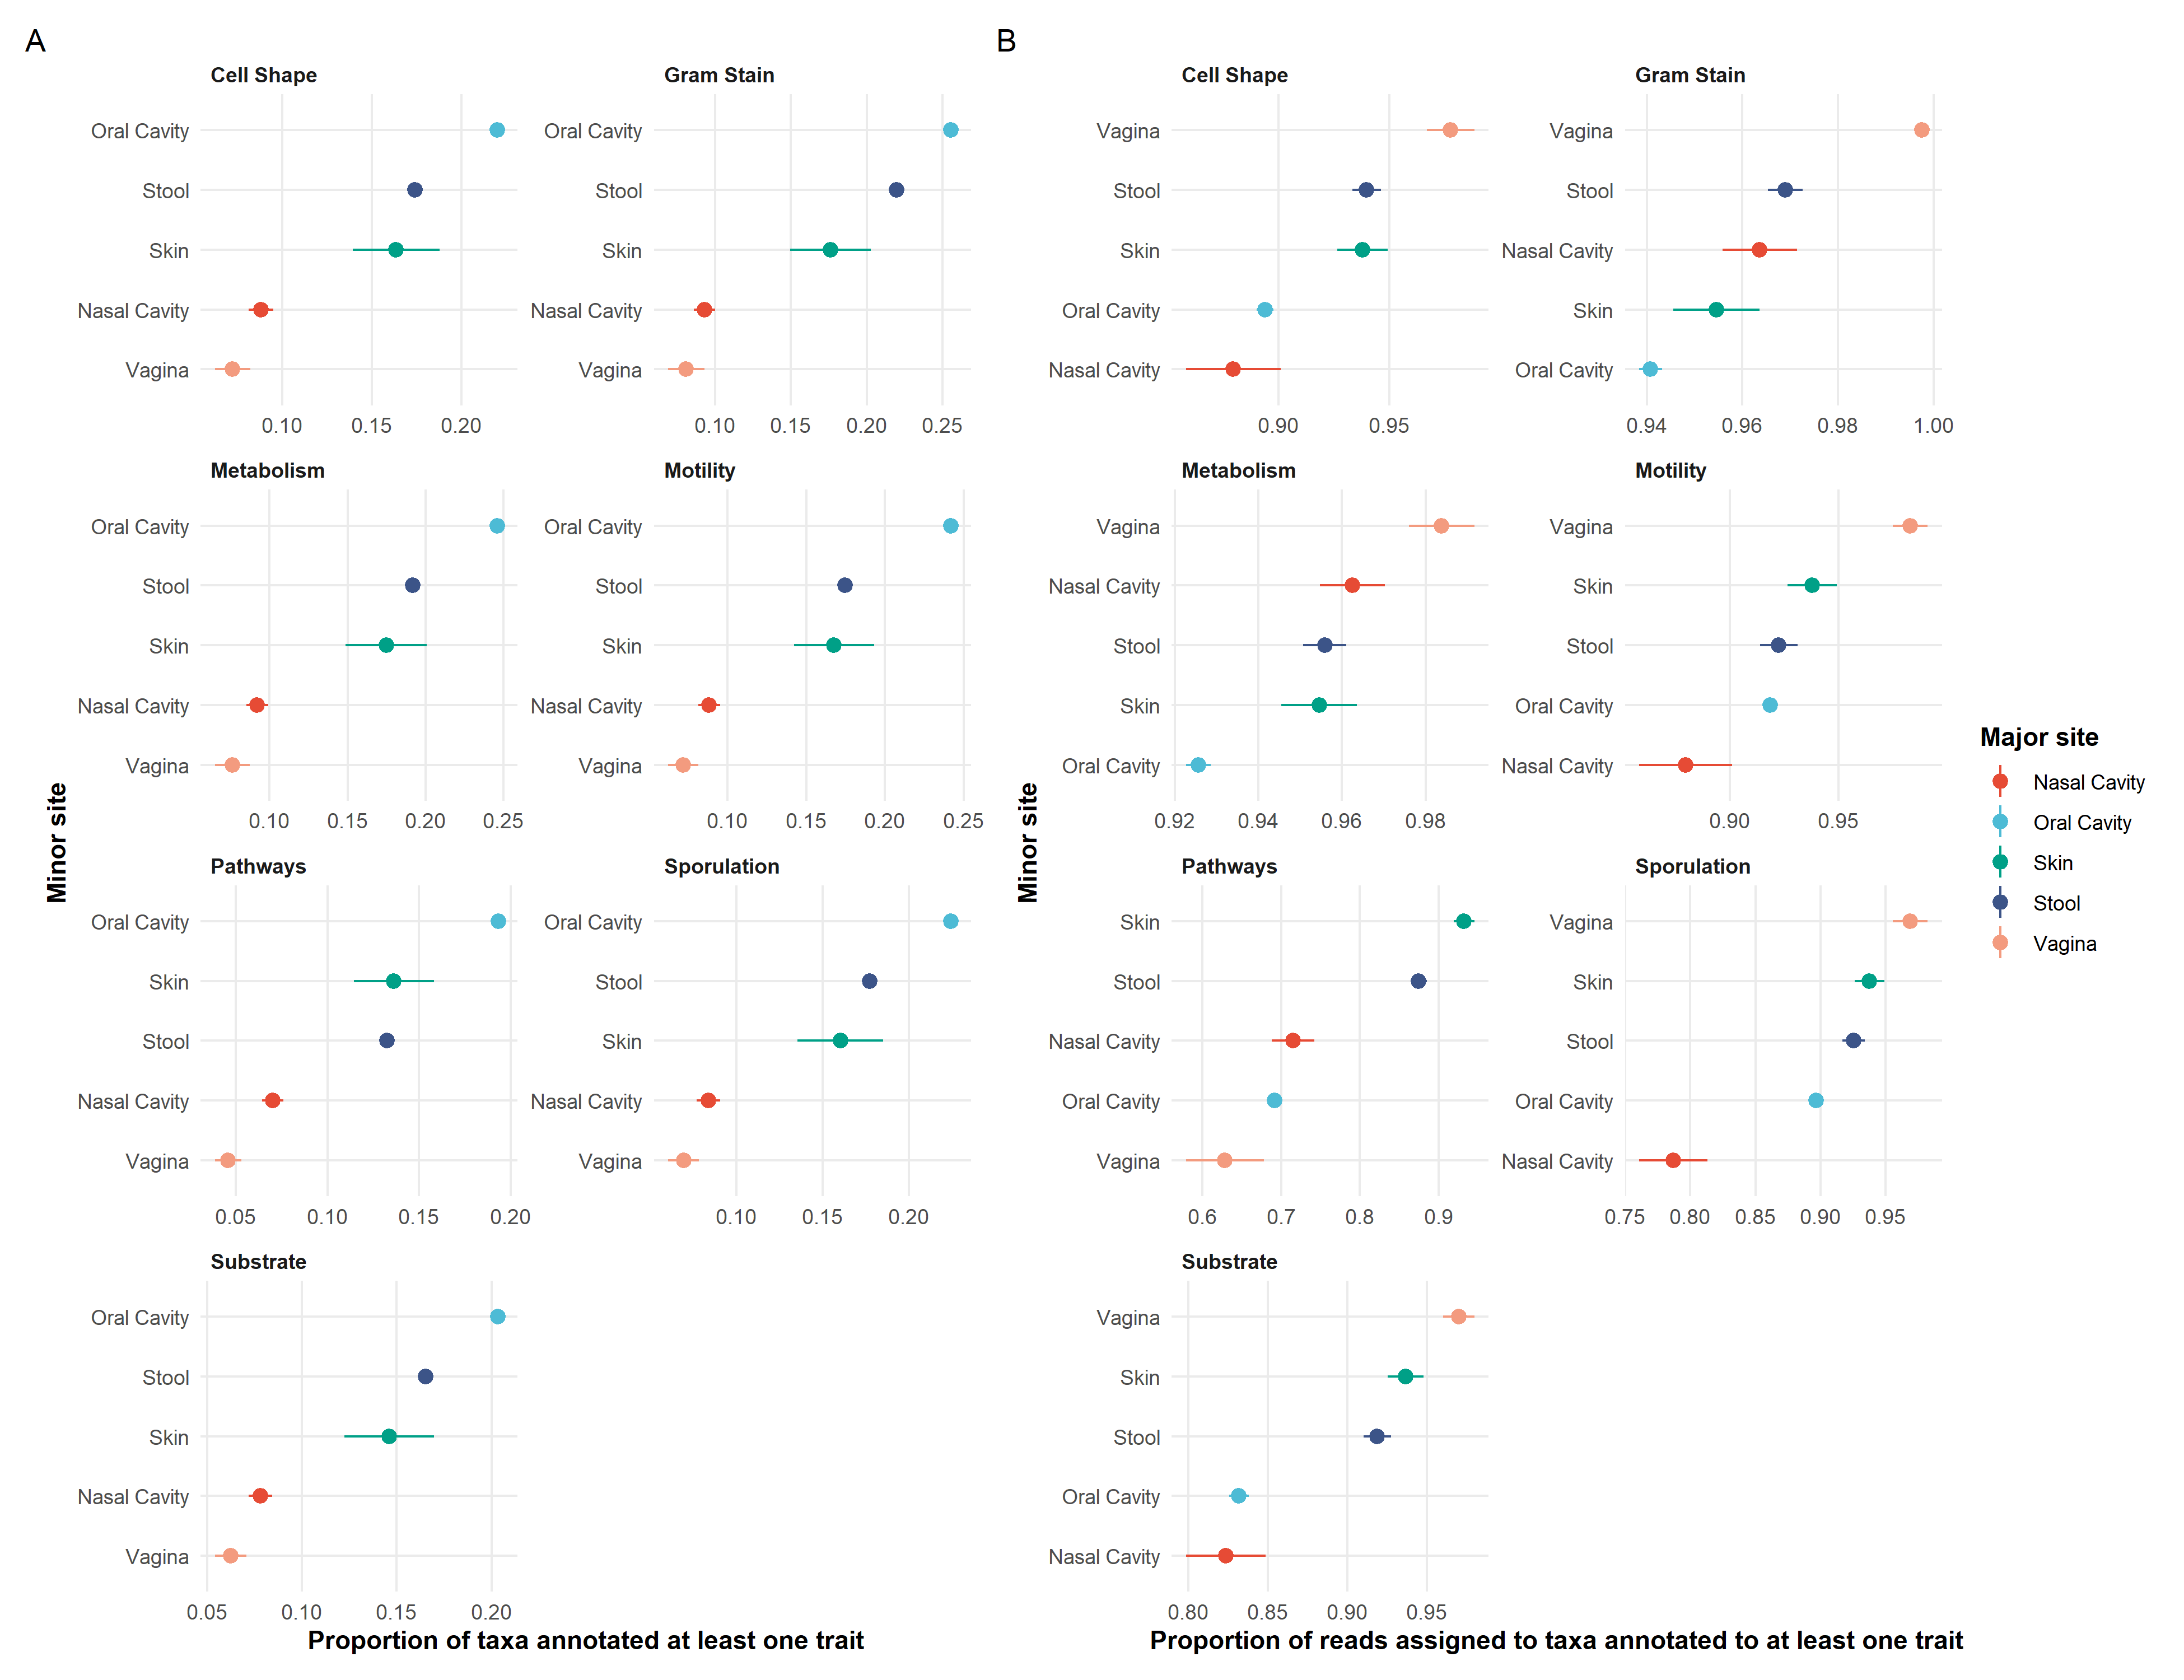
\includegraphics[width=0.99\linewidth]{figures/coverage_wgs.png}
\caption{Trait annotation coverage across different body sites for the HMP data set profiled using whole genome shotgun sequencing. Panel \textbf{(A)} illustrates the proportion of present taxa per sample annotated to at least one trait. Panel \textbf{(B)} illustrates the proportion of reads assigned to taxa annotated to at least one trait which accounts for taxa relative abundances. Each plot facet represents different trait categories that were evaluated}
\label{fig:1}
\end{figure}

\begin{figure}[!h]
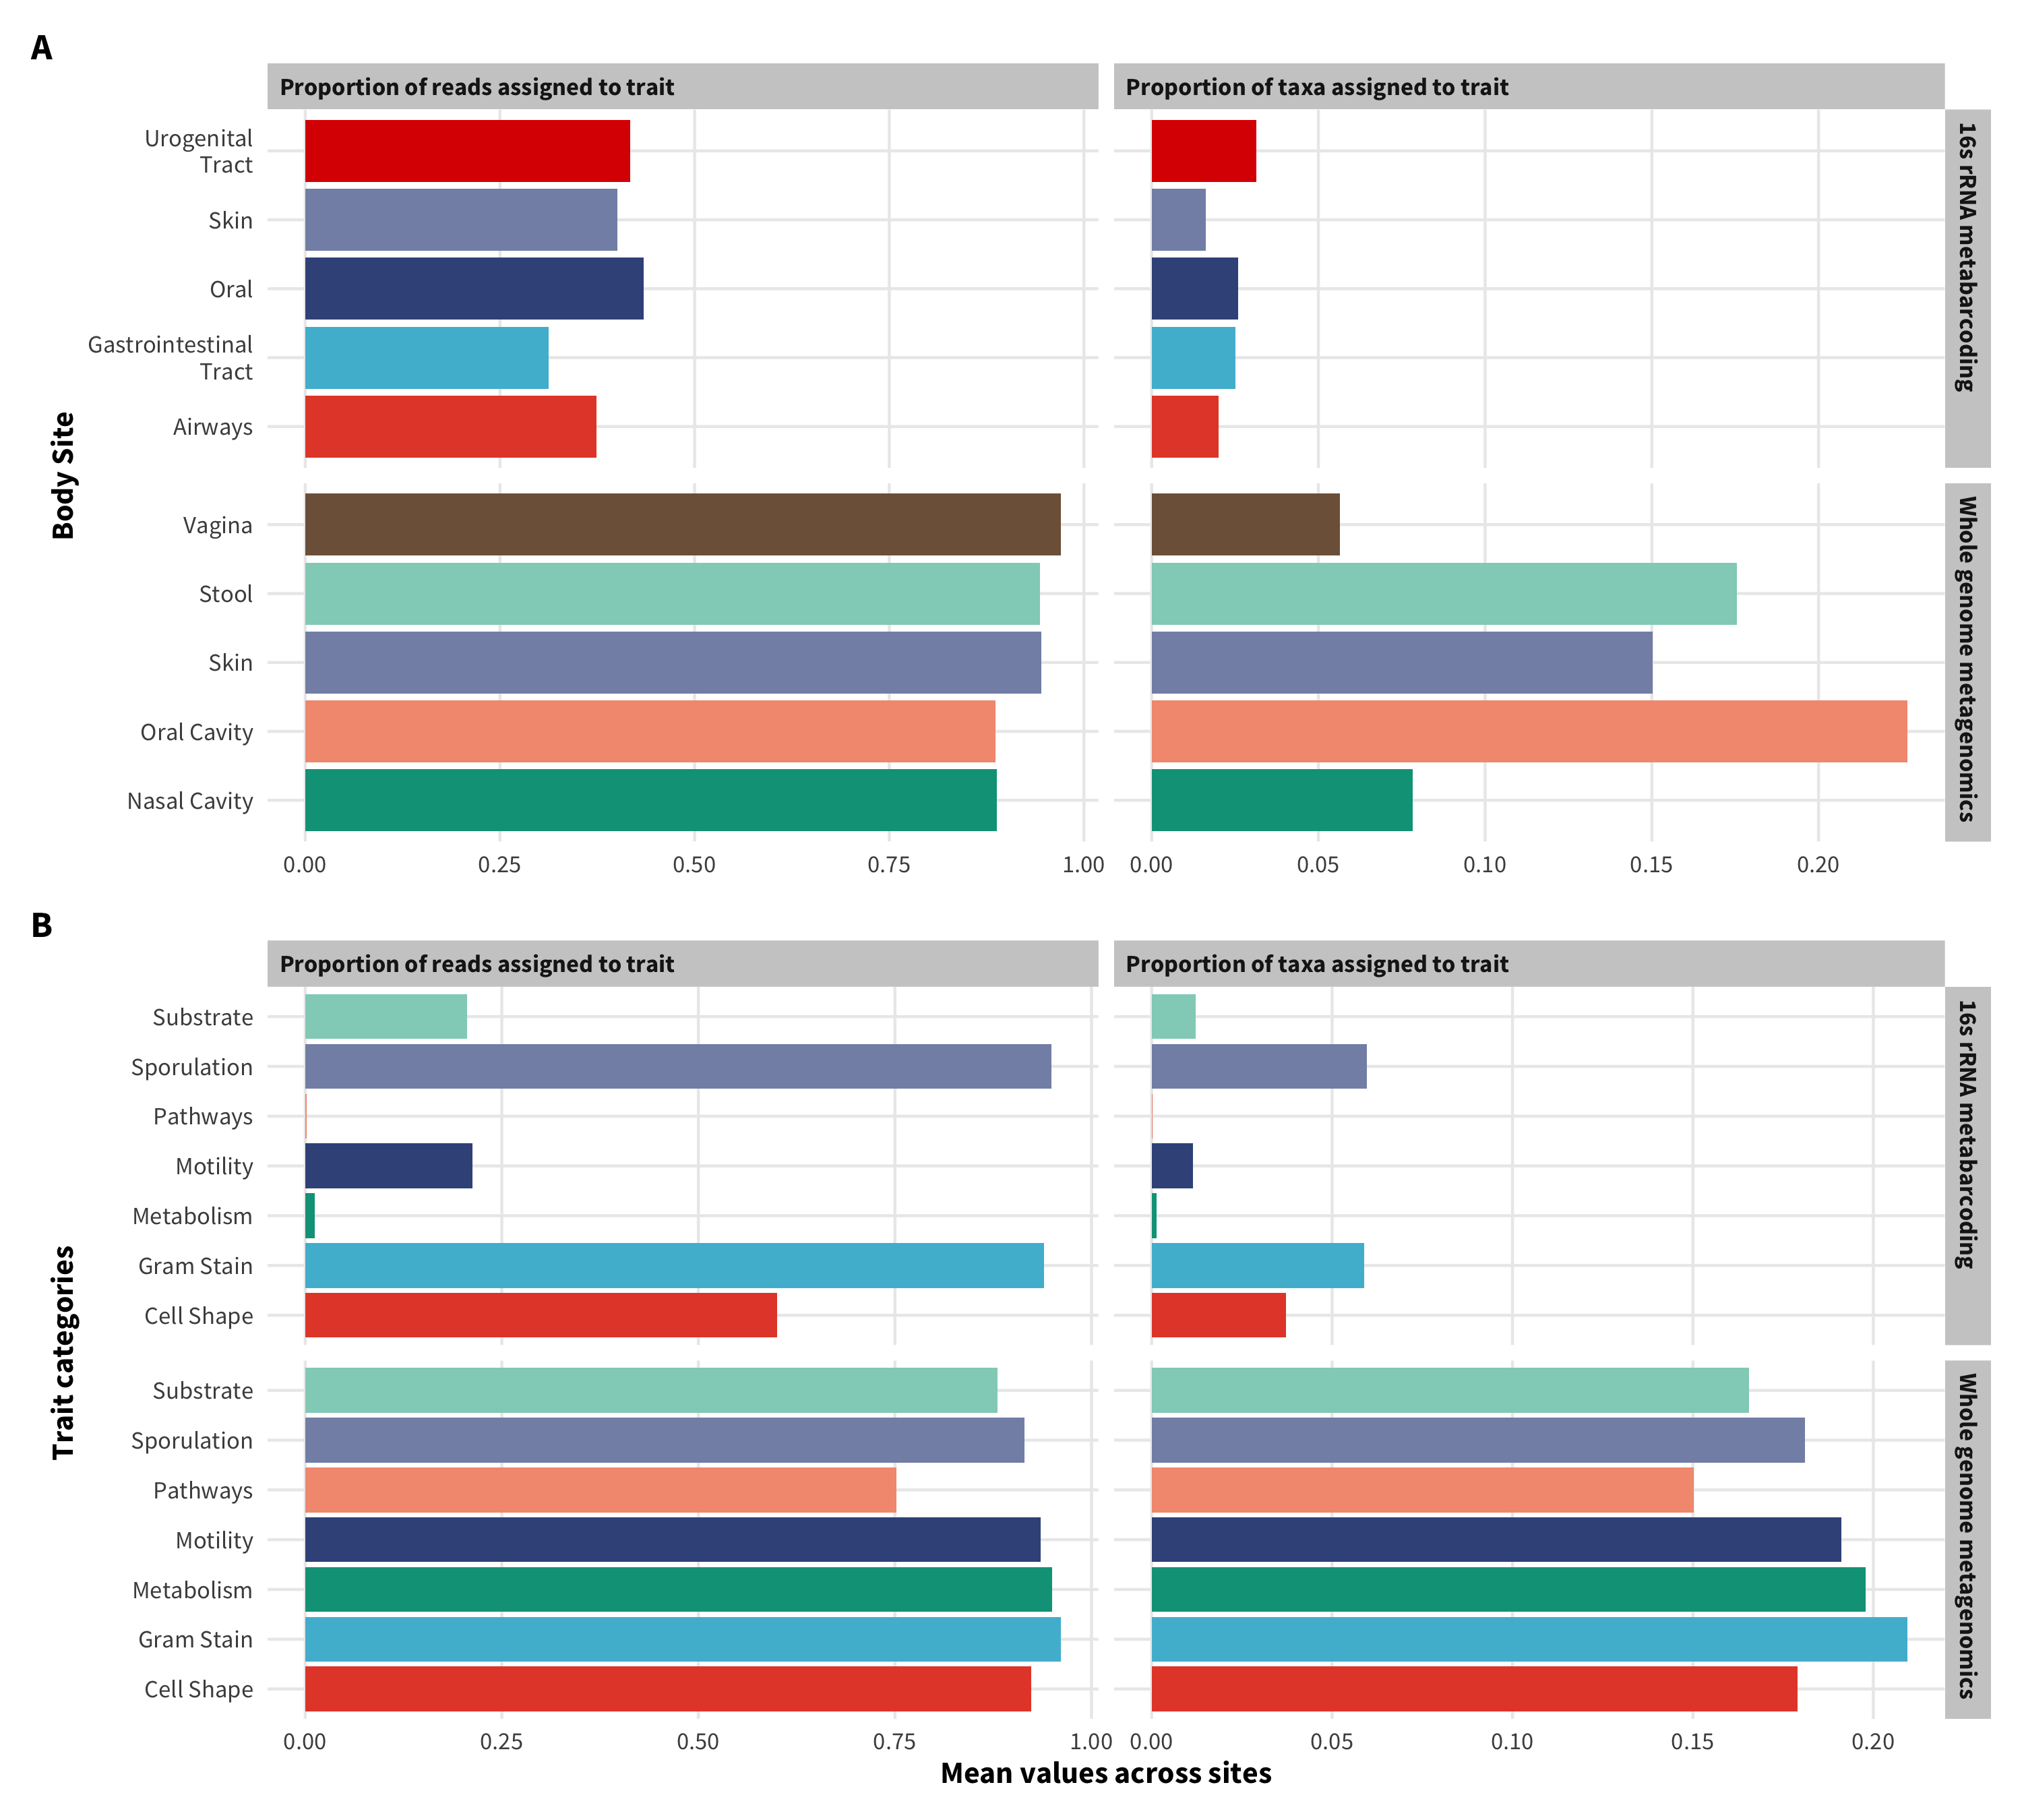
\includegraphics[width=0.99\linewidth]{figures/coverage_by_joint_agg.png}
\caption{Trait annotation coverage across different body sites for the HMP data set profiled using whole genome shotgun sequencing. Panel \textbf{(A)} illustrates the proportion of present taxa per sample annotated to at least one trait. Panel \textbf{(B)} illustrates the proportion of reads assigned to taxa annotated to at least one trait which accounts for taxa relative abundances. Each plot facet represents different trait categories that were evaluated}
\label{fig:2}
\end{figure}

\subsection*{Predictive analysis} 

\begin{figure}[!h]
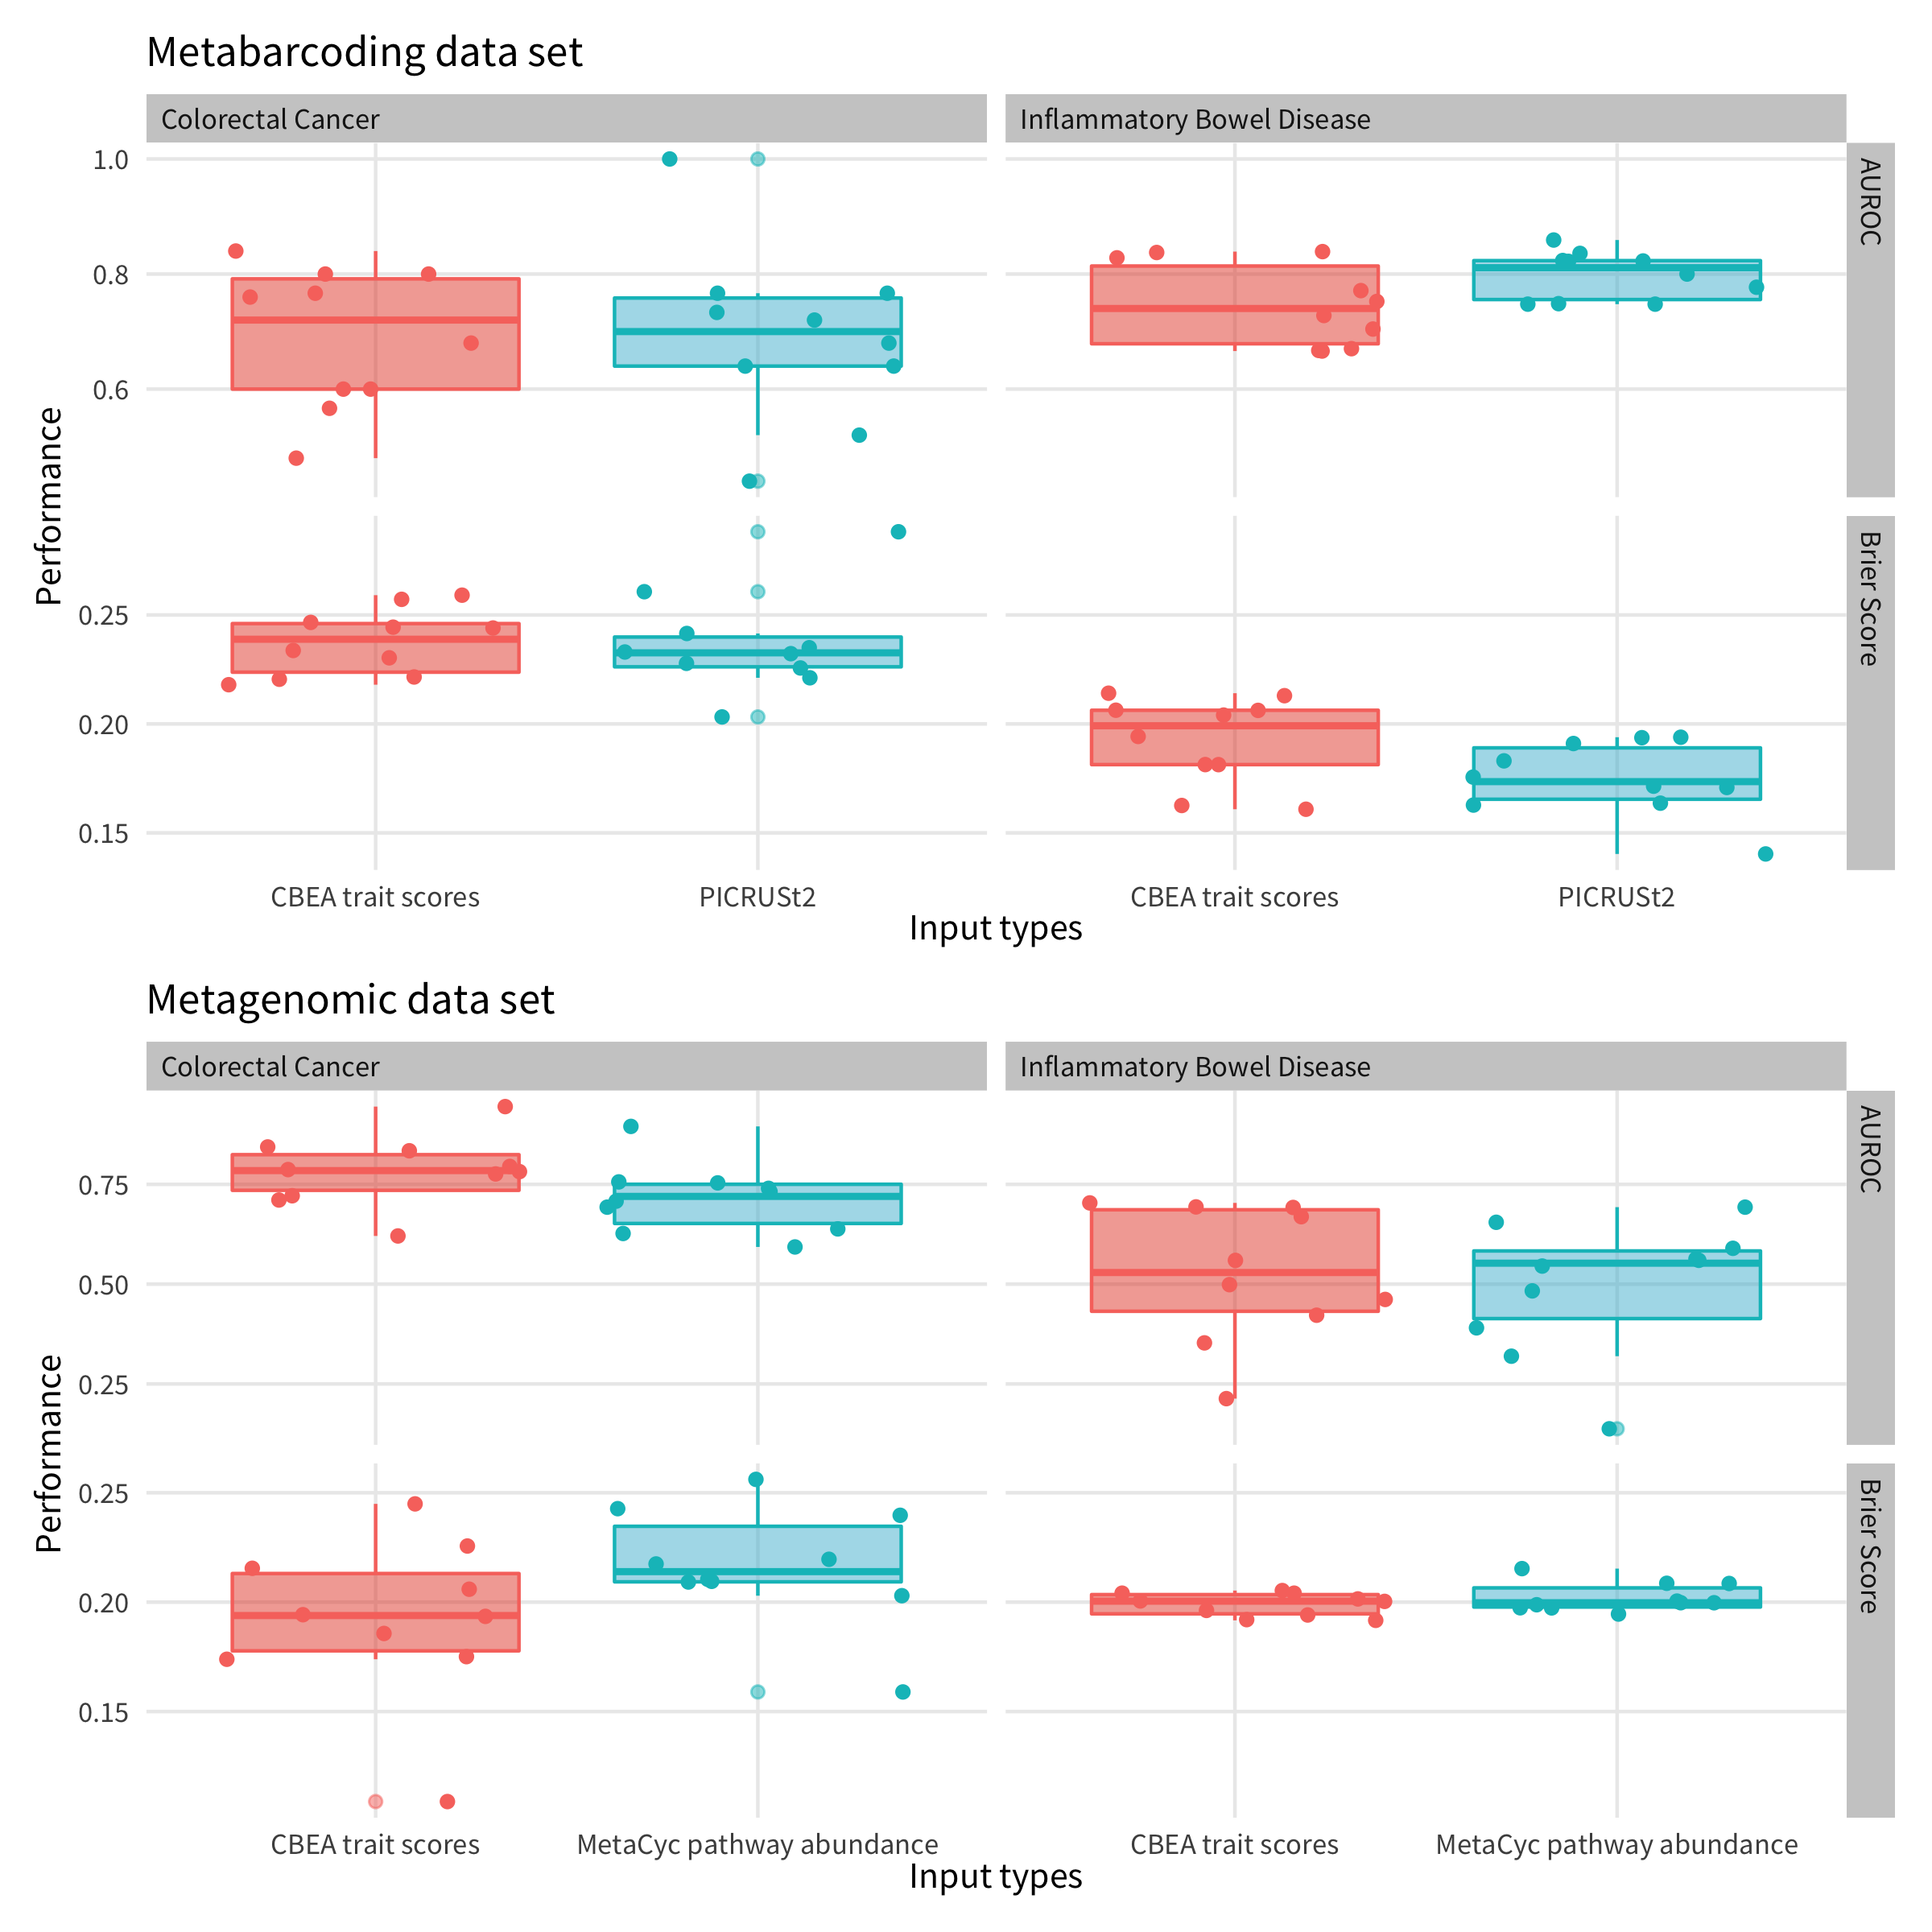
\includegraphics[width=0.99\linewidth]{figures/pred_performance.png}
\caption{Trait annotation coverage across different body sites for the HMP data set profiled using whole genome shotgun sequencing. Panel \textbf{(A)} illustrates the proportion of present taxa per sample annotated to at least one trait. Panel \textbf{(B)} illustrates the proportion of reads assigned to taxa annotated to at least one trait which accounts for taxa relative abundances. Each plot facet represents different trait categories that were evaluated}
\label{fig:3}
\end{figure}

\begin{figure}[!h]
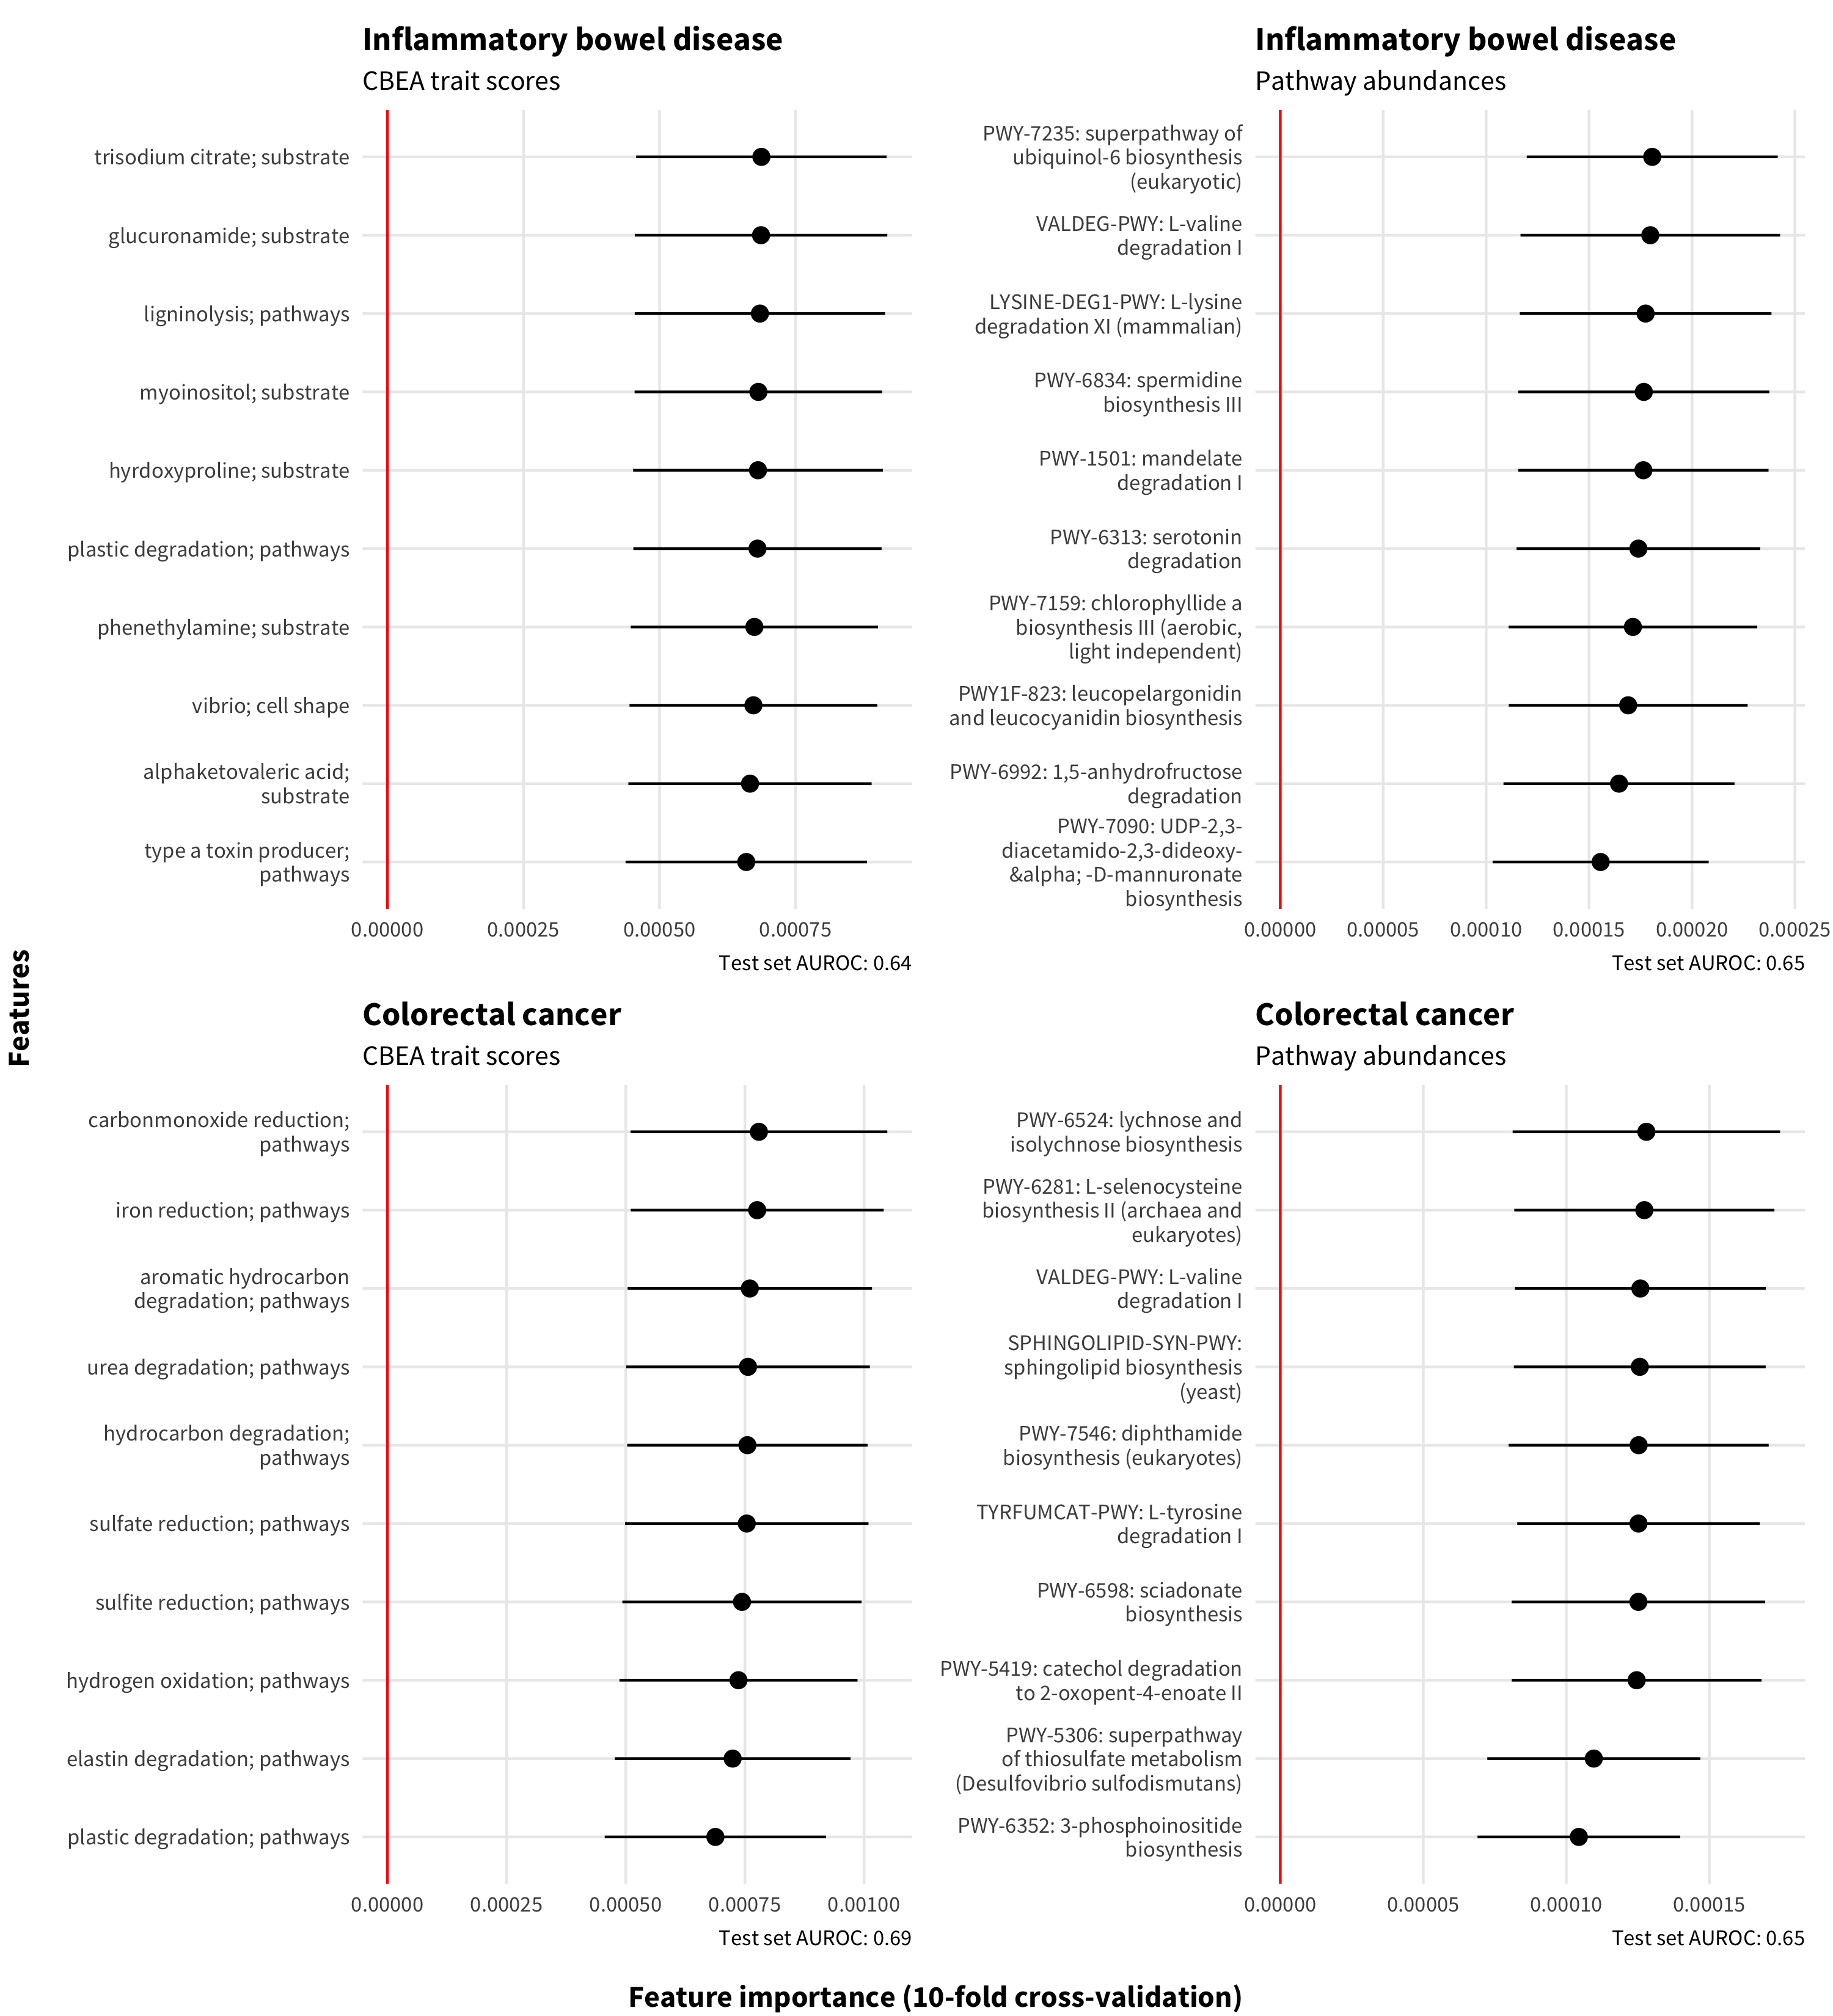
\includegraphics[width=0.99\linewidth]{figures/feat_importance_wgs.png}
\caption{Trait annotation coverage across different body sites for the HMP data set profiled using whole genome shotgun sequencing. Panel \textbf{(A)} illustrates the proportion of present taxa per sample annotated to at least one trait. Panel \textbf{(B)} illustrates the proportion of reads assigned to taxa annotated to at least one trait which accounts for taxa relative abundances. Each plot facet represents different trait categories that were evaluated}
\label{fig:4}
\end{figure}



\subsection*{Concordance with external sources}  


\section*{Discussion}


\section*{Appendix}
Text for this section\ldots

%%%%%%%%%%%%%%%%%%%%%%%%%%%%%%%%%%%%%%%%%%%%%%
%%                                          %%
%% Backmatter begins here                   %%
%%                                          %%
%%%%%%%%%%%%%%%%%%%%%%%%%%%%%%%%%%%%%%%%%%%%%%
\clearpage
\begin{backmatter}

\section*{Acknowledgements}%% if any
We would like to acknowledge Dr. Becky Lebeaux, Dr. Levi Waldron, Dr. Margaret Karagas, and Dr. Brock Christensen for their comments on this manuscript. 

\section*{Funding}%% if any
Text for this section\ldots

\section*{Abbreviations}%% if any
CRC: Colorectal Cancer \\
HMP: Human Microbiome Project \\ 
IBD: Inflammatory Bowel Disease \\
CBEA: Competitive Balances for Taxonomic Enrichment Analysis \\
ENA: European Nucleotide Archive \\

\section*{Availability of data and materials}%% if any
All data for this manuscript is publicly available either via ENA projects () or the \texttt{curatedMetagenomicData} and \texttt{HMP16SData} R packages. Reproducible scripts are also available on GitHub at \texttt{https://www.github.com/qpmnguyen/microbe\_set\_trait}

\section*{Ethics approval and consent to participate}%% if any
Text for this section\ldots

\section*{Competing interests}
The authors declare that they have no competing interests.

\section*{Consent for publication}%% if any
Text for this section\ldots

\section*{Authors' contributions}
QPN, AGH, and HRF conceived of the manuscript and planned the experiments. QPN performed the analyses and wrote up the manuscript. QPN, AGH, and HRF contributed to improving and revising the manuscript.  

\section*{Authors' information}%% if any
Text for this section\ldots

%%%%%%%%%%%%%%%%%%%%%%%%%%%%%%%%%%%%%%%%%%%%%%%%%%%%%%%%%%%%%
%%                  The Bibliography                       %%
%%                                                         %%
%%  Bmc_mathpys.bst  will be used to                       %%
%%  create a .BBL file for submission.                     %%
%%  After submission of the .TEX file,                     %%
%%  you will be prompted to submit your .BBL file.         %%
%%                                                         %%
%%                                                         %%
%%  Note that the displayed Bibliography will not          %%
%%  necessarily be rendered by Latex exactly as specified  %%
%%  in the online Instructions for Authors.                %%
%%                                                         %%
%%%%%%%%%%%%%%%%%%%%%%%%%%%%%%%%%%%%%%%%%%%%%%%%%%%%%%%%%%%%%

% if your bibliography is in bibtex format, use those commands:
\bibliographystyle{bmc-mathphys} % Style BST file (bmc-mathphys, vancouver, spbasic).
\bibliography{references}      % Bibliography file (usually '*.bib' )
% for author-year bibliography (bmc-mathphys or spbasic)
% a) write to bib file (bmc-mathphys only)
% @settings{label, options="nameyear"}
% b) uncomment next line
%\nocite{label}

% or include bibliography directly:
% \begin{thebibliography}
% \bibitem{b1}
% \end{thebibliography}

%%%%%%%%%%%%%%%%%%%%%%%%%%%%%%%%%%%
%%                               %%
%% Figures                       %%
%%                               %%
%% NB: this is for captions and  %%
%% Titles. All graphics must be  %%
%% submitted separately and NOT  %%
%% included in the Tex document  %%
%%                               %%
%%%%%%%%%%%%%%%%%%%%%%%%%%%%%%%%%%%

%%
%% Do not use \listoffigures as most will included as separate files

%\section*{Figures}
%  \begin{figure}[h!]
%  \caption{Sample figure title}
%\end{figure}

%\begin{figure}[h!]
%  \caption{Sample figure title}
%\end{figure}

%%%%%%%%%%%%%%%%%%%%%%%%%%%%%%%%%%%
%%                               %%
%% Tables                        %%
%%                               %%
%%%%%%%%%%%%%%%%%%%%%%%%%%%%%%%%%%%

%% Use of \listoftables is discouraged.
%%
\section*{Tables}
\begin{table}[h!]
\caption{Sample table title. This is where the description of the table should go}
  \begin{tabular}{cccc}
    \hline
    & B1  &B2   & B3\\ \hline
    A1 & 0.1 & 0.2 & 0.3\\
    A2 & ... & ..  & .\\
    A3 & ..  & .   & .\\ \hline
  \end{tabular}
\end{table}

%%%%%%%%%%%%%%%%%%%%%%%%%%%%%%%%%%%
%%                               %%
%% Additional Files              %%
%%                               %%
%%%%%%%%%%%%%%%%%%%%%%%%%%%%%%%%%%%

\section*{Additional Files}
  \subsection*{Additional file 1 --- Sample additional file title}
    Additional file descriptions text (including details of how to
    view the file, if it is in a non-standard format or the file extension).  This might
    refer to a multi-page table or a figure.

  \subsection*{Additional file 2 --- Sample additional file title}
    Additional file descriptions text.

\end{backmatter}
\end{document}
